\documentclass{article} 

\usepackage{fancyhdr}
\usepackage[english]{babel}

\usepackage{fullpage}
\usepackage[margin = .75 in]{geometry}
\usepackage[leqno]{amsmath}
\usepackage{amsmath}
\usepackage{amsfonts}
\usepackage{amssymb}
\usepackage{amsthm}
\usepackage{amssymb}
\usepackage[all]{xy}
\usepackage{graphicx}

\usepackage{graphicx,color,url,hyperref}
\usepackage{epsfig}
\fancyhf{}
\setlength{\parindent}{0pt}
\setlength{\parskip}{5pt plus 1pt}
\setlength{\headheight}{13.6pt}

\newcommand{\NN}{\mathbf N}
\newcommand{\RR}{\mathbf R}
\newcommand{\CC}{\mathbf C}
\newcommand{\ZZ}{\mathbf Z}
\newcommand{\ZZn}[1]{\ZZ/{#1}\ZZ}
\newcommand{\QQ}{\mathbf Q}
\newcommand{\nn}{\mathbb N}
\newcommand{\rr}{\mathbb R}
\newcommand{\cc}{\mathbb C}
\newcommand{\zz}{\mathbb Z}
\newcommand{\zzn}[1]{\zz/{#1}\zz}
\newcommand{\qq}{\mathbb Q}
\newcommand{\calM}{\mathcal M}
\newcommand{\latex}{\LaTeX}
\newcommand{\tex}{\TeX}
\newcommand{\dd}{{\rm d}}
\newcommand{\sm}{\setminus} 

\title{Homework 3}
\author{Sunny Lee}
\date{March 30, 2021}

\pagestyle{fancy}
\fancyhf{}
\rhead{March 30, 2021}
\lhead{Sunny Lee}
\chead{Homework 3}
\rfoot{Page \thepage}

\begin{document}

\begin{enumerate}
    \item Using the Gaussian Elimination method, we obtain the values $x_1 = 3.6480, 
    x_2 = 6.0594, x_3 = -4.1321, x_4 = 4.1755, x_5 = -1.1407$: \\
    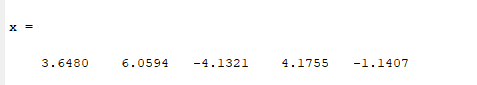
\includegraphics{1.png}

    \item Using the Scaled Partial Pivoting algorithm, we obtain the values $x_1 = 3, 
    x_2 = 1, x_3 = -2, x_4 = 1$. \\
    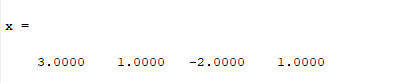
\includegraphics{2.png}

    \item Using the LU decomposition: \\
    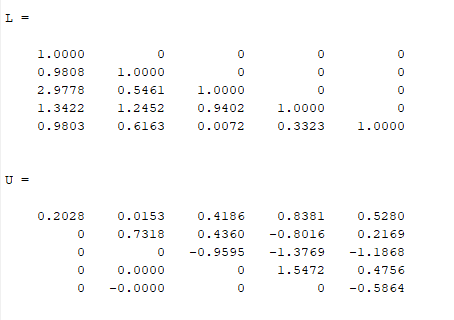
\includegraphics{3a.png}\\
    Using this decomposition to solve for $x$: \\
    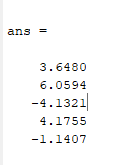
\includegraphics{3b.png}\\
    which is the same vector we obtained in question 1. 
\pagebreak
    \item In order to check to see if this matrix is positive definite, we can check 
    if the determinant of its leading principal submatrices are all positive:\\
    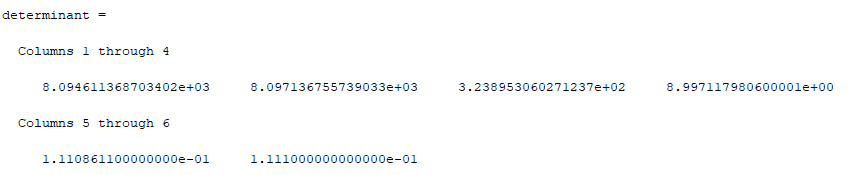
\includegraphics[scale = .8]{4a.png}\\
    Since all of the determinants above are positive, we conclude that $A$ is a 
    positive definite matrix. Using the Cholesky algorithm, we obtain the Upper 
    triangular matrix: \\
    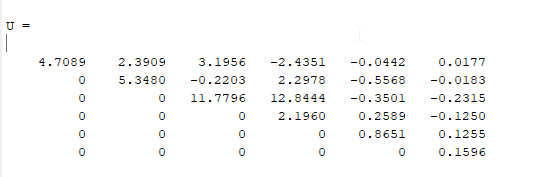
\includegraphics{4b.png}\\
    and since $A = U^TU$, we can take the inverse of $U^TU$ and multiply them 
    on both sides to solve our equation:\\
    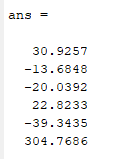
\includegraphics{4c.png}\\
\pagebreak
    \item Running the LDL factorization, we obtain these matrices: \\
    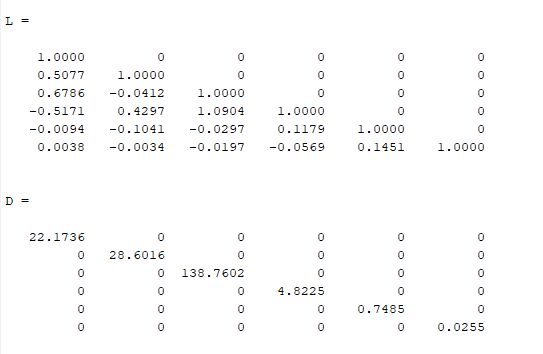
\includegraphics{5a.png}\\
    By taking the inverse of the $LDL^T$, we can find the solution to our equation: \\
    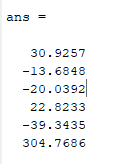
\includegraphics{5b.png}\\

    \item 
    \begin{enumerate}
        \item 
        \begin{gather*}
            M_1^{-1}M_2^{-1} = (M_2 M_1)^{-1} \\
            M_2 M_1 = 
            \begin{bmatrix}
                1 & 0 & 0\\
                m_{21} & 1 & 0\\
                m_{32}m_{21}+m_{31} & m_{32} & 1
            \end{bmatrix}
        \end{gather*}
        Calculating the matrix of cofactors: 
        \begin{gather*}
            \begin{bmatrix}
                1 & -m_{21} & -m_{31}\\
                0 & 1 & -m_{32}\\
                0 & 0 & 1
            \end{bmatrix}
        \end{gather*}
        Since the original matrix is lower triangular, we can multiply the diagonals of that 
        matrix and we get $det(M_2 M_1) = 1$. Thus, we transpose the matrix of cofactors: 
        \begin{gather*}
            \begin{bmatrix}
                1 & 0 & 0\\
                -m_{21} & 1 & 0\\
                -m_{31} & -m_{32} & 1
            \end{bmatrix}
        \end{gather*}

        \item From the matrix given, we can perform elimination on the matrix to 
        get the pivots: 
        \begin{gather*}
            \begin{bmatrix}
                1 & a\\
                0 & 1-a^2
            \end{bmatrix}
        \end{gather*}
        To make the matrix positive definite, we must have $1-a^2 \leq 0$. Thus, we see
        that the matrix $A$ is not positive definite for all $|a| \geq 1$. 

        \item Since the determinant of $A$ is 55, $A$ is invertible. 

        \item Using the LDL factorization and looking at the diagonal matrix: \\
        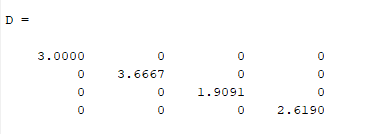
\includegraphics{6d.png}\\
        Since all of the values are positive, we conclude that the matrix itself is 
        positive definite. 
    \end{enumerate}
    
    \item 
    \begin{enumerate}
        \item
        Finding the determinant of the matrix: \\
        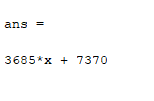
\includegraphics{7a.png}\\
        and setting the determinant equal to zero, we find that $x = 2$.

        \item Since the determinant of the matrix is $-1$ which is not zero, we can 
        find the inverse of the matrix: \\
        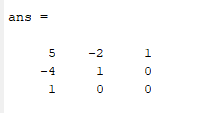
\includegraphics{7b.png}

        \item 
        Since $7 > 2 + 3$, $6 > 4 + 1$ and $5 > 2 + 1$, we can say that $A$ is 
        strictly diagonally dominant. Since $A$ is strictly diagonally dominant, 
        $A$ is nonsingular. Gaussian Elimination cannot be performed on any linear 
        system without row or column changes since there will be times where the 
        current pivot is zero while other rows below have non zero values for that 
        column. 

        \item 
        The inverse of $A$: \\
        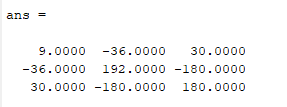
\includegraphics{7d.png}\\
        Calculating the determinant of $A^{100}$, we find that the determinant
        is not zero, and thus $A^{100}$ is invertible. 
    \end{enumerate}

    \item Setting up the iterative form of the Jacobi Method: 
    \begin{gather*}
        x^{(k)} =
        \begin{bmatrix}
            0 & \frac{1}{3} & -\frac{1}{3}\\
            -\frac{1}{2} & 0 & -\frac{1}{3}\\
            -\frac{3}{7} & -\frac{3}{7} & 0
        \end{bmatrix}
        x^{(k-1)} + 
        \begin{bmatrix}
            \frac{1}{3}\\
            0\\
            \frac{4}{7}
        \end{bmatrix}
    \end{gather*}
\pagebreak
    Using this method in MATLAB, we get these approximations for the first two
    iterations: \\
    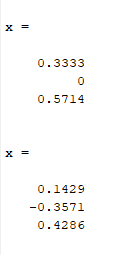
\includegraphics{8.png}\\

    \item Running the Gauss Seidel method, our first two iterations yield: \\
    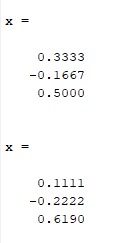
\includegraphics{9.png}

    \item To find $||A||_{\infty}$, we take the maximum of the sum of the absolute
    values of each row of $A$, thus: $||A||_{\infty} = max(3, 3, 3) = 3$. To find 
    the $||A||_2$, we use the $l_2$ norm for vectors on each row, thus $||A||_2 = 
    max(\sqrt{5}, \sqrt{5}, 3) = 3$. 

\end{enumerate}

\end{document}